% Options for packages loaded elsewhere
\PassOptionsToPackage{unicode}{hyperref}
\PassOptionsToPackage{hyphens}{url}
\documentclass[
  english,
]{article}
\usepackage{xcolor}
\usepackage{amsmath,amssymb}
\setcounter{secnumdepth}{5}
\usepackage{iftex}
\ifPDFTeX
  \usepackage[T1]{fontenc}
  \usepackage[utf8]{inputenc}
  \usepackage{textcomp} % provide euro and other symbols
\else % if luatex or xetex
  \usepackage{unicode-math} % this also loads fontspec
  \defaultfontfeatures{Scale=MatchLowercase}
  \defaultfontfeatures[\rmfamily]{Ligatures=TeX,Scale=1}
\fi
% \usepackage{lmodern}
\ifPDFTeX\else
  % xetex/luatex font selection
\fi
% Use upquote if available, for straight quotes in verbatim environments
\IfFileExists{upquote.sty}{\usepackage{upquote}}{}
\IfFileExists{microtype.sty}{% use microtype if available
  \usepackage[]{microtype}
  \UseMicrotypeSet[protrusion]{basicmath} % disable protrusion for tt fonts
}{}
\makeatletter
\@ifundefined{KOMAClassName}{% if non-KOMA class
  \IfFileExists{parskip.sty}{%
    \usepackage{parskip}
  }{% else
    \setlength{\parindent}{0pt}
    \setlength{\parskip}{6pt plus 2pt minus 1pt}}
}{% if KOMA class
  \KOMAoptions{parskip=half}}
\makeatother
\usepackage{color}
\usepackage{fancyvrb}
\newcommand{\VerbBar}{|}
\newcommand{\VERB}{\Verb[commandchars=\\\{\}]}
\DefineVerbatimEnvironment{Highlighting}{Verbatim}{commandchars=\\\{\}}
% Add ',fontsize=\small' for more characters per line
\newenvironment{Shaded}{}{}
\newcommand{\AlertTok}[1]{\textcolor[rgb]{1.00,0.00,0.00}{\textbf{#1}}}
\newcommand{\AnnotationTok}[1]{\textcolor[rgb]{0.38,0.63,0.69}{\textbf{\textit{#1}}}}
\newcommand{\AttributeTok}[1]{\textcolor[rgb]{0.49,0.56,0.16}{#1}}
\newcommand{\BaseNTok}[1]{\textcolor[rgb]{0.25,0.63,0.44}{#1}}
\newcommand{\BuiltInTok}[1]{\textcolor[rgb]{0.00,0.50,0.00}{#1}}
\newcommand{\CharTok}[1]{\textcolor[rgb]{0.25,0.44,0.63}{#1}}
\newcommand{\CommentTok}[1]{\textcolor[rgb]{0.38,0.63,0.69}{\textit{#1}}}
\newcommand{\CommentVarTok}[1]{\textcolor[rgb]{0.38,0.63,0.69}{\textbf{\textit{#1}}}}
\newcommand{\ConstantTok}[1]{\textcolor[rgb]{0.53,0.00,0.00}{#1}}
\newcommand{\ControlFlowTok}[1]{\textcolor[rgb]{0.00,0.44,0.13}{\textbf{#1}}}
\newcommand{\DataTypeTok}[1]{\textcolor[rgb]{0.56,0.13,0.00}{#1}}
\newcommand{\DecValTok}[1]{\textcolor[rgb]{0.25,0.63,0.44}{#1}}
\newcommand{\DocumentationTok}[1]{\textcolor[rgb]{0.73,0.13,0.13}{\textit{#1}}}
\newcommand{\ErrorTok}[1]{\textcolor[rgb]{1.00,0.00,0.00}{\textbf{#1}}}
\newcommand{\ExtensionTok}[1]{#1}
\newcommand{\FloatTok}[1]{\textcolor[rgb]{0.25,0.63,0.44}{#1}}
\newcommand{\FunctionTok}[1]{\textcolor[rgb]{0.02,0.16,0.49}{#1}}
\newcommand{\ImportTok}[1]{\textcolor[rgb]{0.00,0.50,0.00}{\textbf{#1}}}
\newcommand{\InformationTok}[1]{\textcolor[rgb]{0.38,0.63,0.69}{\textbf{\textit{#1}}}}
\newcommand{\KeywordTok}[1]{\textcolor[rgb]{0.00,0.44,0.13}{\textbf{#1}}}
\newcommand{\NormalTok}[1]{#1}
\newcommand{\OperatorTok}[1]{\textcolor[rgb]{0.40,0.40,0.40}{#1}}
\newcommand{\OtherTok}[1]{\textcolor[rgb]{0.00,0.44,0.13}{#1}}
\newcommand{\PreprocessorTok}[1]{\textcolor[rgb]{0.74,0.48,0.00}{#1}}
\newcommand{\RegionMarkerTok}[1]{#1}
\newcommand{\SpecialCharTok}[1]{\textcolor[rgb]{0.25,0.44,0.63}{#1}}
\newcommand{\SpecialStringTok}[1]{\textcolor[rgb]{0.73,0.40,0.53}{#1}}
\newcommand{\StringTok}[1]{\textcolor[rgb]{0.25,0.44,0.63}{#1}}
\newcommand{\VariableTok}[1]{\textcolor[rgb]{0.10,0.09,0.49}{#1}}
\newcommand{\VerbatimStringTok}[1]{\textcolor[rgb]{0.25,0.44,0.63}{#1}}
\newcommand{\WarningTok}[1]{\textcolor[rgb]{0.38,0.63,0.69}{\textbf{\textit{#1}}}}
\usepackage{longtable,booktabs,array}
\usepackage{caption}
\captionsetup[table]{skip=6pt}
\newcounter{none} % for unnumbered tables
\usepackage{calc} % for calculating minipage widths
% Correct order of tables after \paragraph or \subparagraph
\usepackage{etoolbox}
\makeatletter
\patchcmd\longtable{\par}{\if@noskipsec\mbox{}\fi\par}{}{}
\makeatother
% Allow footnotes in longtable head/foot
\IfFileExists{footnotehyper.sty}{\usepackage{footnotehyper}}{\usepackage{footnote}}
\makesavenoteenv{longtable}
\usepackage{graphicx}
\makeatletter
\newsavebox\pandoc@box
\newcommand*\pandocbounded[1]{% scales image to fit in text height/width
  \sbox\pandoc@box{#1}%
  \Gscale@div\@tempa{\textheight}{\dimexpr\ht\pandoc@box+\dp\pandoc@box\relax}%
  \Gscale@div\@tempb{\linewidth}{\wd\pandoc@box}%
  \ifdim\@tempb\p@<\@tempa\p@\let\@tempa\@tempb\fi% select the smaller of both
  \ifdim\@tempa\p@<\p@\scalebox{\@tempa}{\usebox\pandoc@box}%
  \else\usebox{\pandoc@box}%
  \fi%
}
% Set default figure placement to htbp
\def\fps@figure{htbp}
\makeatother
\ifLuaTeX
\usepackage[bidi=basic,shorthands=off]{babel}
\else
\usepackage[bidi=default,shorthands=off]{babel}
\fi
\ifLuaTeX
  \usepackage{selnolig} % disable illegal ligatures
\fi
\setlength{\emergencystretch}{3em} % prevent overfull lines
\providecommand{\tightlist}{%
  \setlength{\itemsep}{0pt}\setlength{\parskip}{0pt}}
\usepackage[]{natbib}
\bibliographystyle{plainnat}
\makeatletter
\@ifpackageloaded{subcaption}{}{\usepackage{subcaption}}
\@ifpackageloaded{caption}{}{\usepackage{caption}}
\captionsetup[subfigure]{margin=0.5em}
\AtBeginDocument{%
\renewcommand*\figurename{Figure}
\renewcommand*\tablename{Table}
}
\AtBeginDocument{%
\renewcommand*\listfigurename{List of Figures}
\renewcommand*\listtablename{List of Tables}
}
\newcounter{pandoccrossref@subfigures@footnote@counter}
\newenvironment{pandoccrossrefsubfigures}{%
\setcounter{pandoccrossref@subfigures@footnote@counter}{0}
\begin{figure}\centering%
\gdef\global@pandoccrossref@subfigures@footnotes{}%
\DeclareRobustCommand{\footnote}[1]{\footnotemark%
\stepcounter{pandoccrossref@subfigures@footnote@counter}%
\ifx\global@pandoccrossref@subfigures@footnotes\empty%
\gdef\global@pandoccrossref@subfigures@footnotes{{##1}}%
\else%
\g@addto@macro\global@pandoccrossref@subfigures@footnotes{, {##1}}%
\fi}}%
{\end{figure}%
\addtocounter{footnote}{-\value{pandoccrossref@subfigures@footnote@counter}}
\@for\f:=\global@pandoccrossref@subfigures@footnotes\do{\stepcounter{footnote}\footnotetext{\f}}%
\gdef\global@pandoccrossref@subfigures@footnotes{}}
\@ifpackageloaded{float}{}{\usepackage{float}}
\floatstyle{ruled}
\@ifundefined{c@chapter}{\newfloat{codelisting}{h}{lop}}{\newfloat{codelisting}{h}{lop}[chapter]}
\floatname{codelisting}{Listing}
\newcommand*\listoflistings{\listof{codelisting}{List of Listings}}
\makeatother
\usepackage{bookmark}
\IfFileExists{xurl.sty}{\usepackage{xurl}}{} % add URL line breaks if available
\urlstyle{same}
% fallback for those not using the hyperref driver hyperxmp:
\makeatletter
\@ifundefined{xmpquote}{\newcommand{\xmpquote}[1]{#1}}{}
\makeatother
\hypersetup{
  pdftitle={Jev in Practice: A Composable Python Toolkit for TypeSafe\textquotesingle s System One Decision Model},
  pdfauthor={Daniel Ari Friedman},
  pdflang={en},
  colorlinks=true,linkcolor=red,urlcolor=red,citecolor=red,anchorcolor=red,filecolor=red,
  pdfcreator={LaTeX via pandoc}}

\title{Jev in Practice: A Composable Python Toolkit for
TypeSafe\textquotesingle s System One Decision Model}
\author{Daniel Ari Friedman}
\date{}

\IfFileExists{seqsplit.sty}{\usepackage{seqsplit}}{\newcommand{\seqsplit}[1]{#1}}
\protected\def\breakseq#1{\seqsplit{#1}}
\protected\def\breaktt#1{\begingroup\ttfamily\seqsplit{#1}\endgroup}
\title{Jev in Practice: A Composable Python Toolkit for TypeSafe's System One Decision Model}
\author{Daniel Ari Friedman}
\date{\today}

% Core mathematics
\usepackage{amsmath}
\usepackage{amssymb}
\usepackage{amsfonts}
\usepackage{amsthm}

% Document layout
\usepackage{geometry}
\geometry{margin=0.25in}
\usepackage{float}
\usepackage{graphicx}

% Tables
\usepackage{booktabs}
\usepackage{longtable}
\usepackage{array}

% Algorithm typesetting (for pseudocode in §2 Methodology)
\IfFileExists{algorithm2e.sty}{\usepackage[ruled,vlined,linesnumbered]{algorithm2e}}{}

% Code listings
\usepackage{listings}

% Typography and formatting
\usepackage{microtype}
\usepackage{xcolor}
\IfFileExists{siunitx.sty}{\usepackage[binary-units]{siunitx}}{}

% Cross-references and citations
\usepackage{hyperref}
\hypersetup{
    colorlinks=true,
    allcolors=red
}
\usepackage[capitalise,noabbrev]{cleveref}
\usepackage{natbib}

% ── Unicode-capable mono font for code listings ──────────────────────
% JuliaMono (TeX Live 2026) covers the full math/Greek glyph set used in
% scientific code blocks; the default lmmono lacks \alpha/\mu/\partial/\nabla.
%
% The hardcoded TeX Live 2026 path below is portable to most macOS / Linux
% TeX Live installs that placed JuliaMono under the default texmf-dist path.
% If your TeX Live version differs (e.g., 2025, 2027) or your distribution
% installs fonts elsewhere, comment out the explicit Path = line — fontspec
% will then search the system font path. If JuliaMono is not installed at
% all, comment out the whole block; xelatex falls back to lmmono with
% reduced Unicode coverage but the document still compiles.
\usepackage{fontspec}
\setmonofont{JuliaMono-Regular}[
  Path           = /usr/local/texlive/2026/texmf-dist/fonts/truetype/public/juliamono/,
  Extension      = .ttf,
  UprightFont    = *,
  BoldFont       = JuliaMono-Bold,
  ItalicFont     = JuliaMono-RegularItalic,
  BoldItalicFont = JuliaMono-BoldItalic,
  Scale          = MatchLowercase,
]

% Math font for unicode-math: Latin Modern Math (TeX Live) has full BMP
% coverage including U+2223 (\mid), U+226A/226B (\ll/\gg), and the Greek/
% blackboard letters used in equations. Without an explicit \setmathfont,
% unicode-math falls back to lmroman text font which lacks several glyphs
% and emits "Missing character" warnings on every \mid in math mode.
\setmathfont{latinmodern-math.otf}
\newtheorem{theorem}{Theorem}[section]
\newtheorem{remark}[theorem]{Remark}
\newtheorem{example}[theorem]{Example}

\begin{document}
\begin{titlepage}
\centering
\vspace*{0.55cm}
{\Huge\sffamily\bfseries Jev in Practice: A Composable Python Toolkit for TypeSafe's System One Decision Model\par}
\vspace{0.4em}
{\Large\sffamily Batching Speedups, Confidence-Gated Routing, and Calibrated Decisions over a Single HTTP Endpoint\par}
\vspace{0.75em}
{\large\sffamily\bfseries Daniel Ari Friedman\par}
{\small\sffamily Active Inference Institute\par}
{\small\sffamily\texttt{daniel@activeinference.institute}\par}
{\small\sffamily\href{https://orcid.org/0000-0001-6232-9096}{ORCID: 0000-0001-6232-9096}\par}
\vspace{0.08em}
{\small\sffamily DOI: \href{https://doi.org/10.5281/zenodo.22816187}{10.5281/zenodo.22816187}\par}
\vspace{0.35em}
\makeatletter
{\@date\par}
\makeatother
\vfill

\includegraphics[width=0.98\textwidth,height=0.6\textheight,keepaspectratio,alt={Graphical abstract, three zones read left to right: the decision state with the noul, choice, and score question primitives; the daf-jev layer stack from typed client through compose gates and routing to the evaluator and calibration, consumed via CLI, MCP server, and agent skill; and a live outputs panel with batching speedups, pipeline latency, and calibration reliability read from the benchmark JSON payloads.}]{\detokenize{../figures/graphical_abstract.png}}
\vfill
\end{titlepage}
\thispagestyle{empty}
\tableofcontents
\newpage

\section{Abstract}\label{sec:abstract}

\begin{figure}
\centering
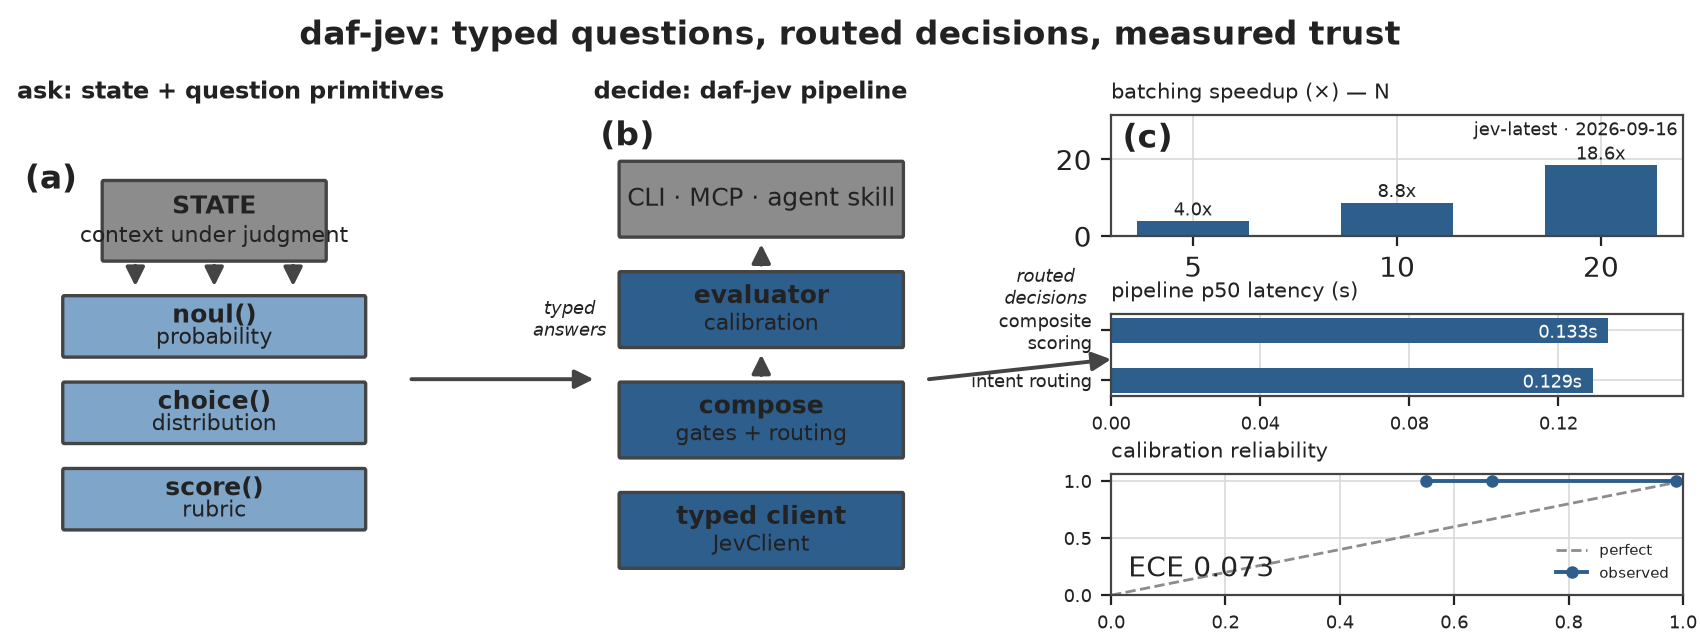
\includegraphics[width=1\linewidth,height=0.5\textheight,keepaspectratio,alt={Graphical abstract for the daf-jev manuscript, in three zones read left to right. Left: the decision state --- the context to be judged --- together with stylized cards for the three typed question primitives: a noul (a 0--1 calibrated probability), a choice (a probability distribution over named options), and a score (a rubric over ordered levels). Center: the package's layer stack, from the typed client through the compose layer's gates and routing to the evaluator and its calibration checks, with the CLI, the MCP server, and the agent skill as consumer surfaces. Right: a live-outputs panel whose batching speedup bars, speedup annotation, pipeline latency figure, and calibration reliability mini-curve are all read from the latest batching, patterns, and calibration benchmark JSON payloads at generation time --- no metric in this panel is hardcoded. Arrows run left to right, tracing the path from an unstructured state to typed answers to composable decisions.}]{../figures/graphical_abstract.png}
\caption{Graphical abstract for the daf-jev manuscript, in three zones
read left to right. Left: the decision \emph{state} --- the context to
be judged --- together with stylized cards for the three typed question
primitives: a \protect\texttt{noul} (a 0--1 calibrated probability), a
\protect\texttt{choice} (a probability distribution over named options),
and a \protect\texttt{score} (a rubric over ordered levels). Center: the
package's layer stack, from the typed client through the compose layer's
gates and routing to the evaluator and its calibration checks, with the
CLI, the MCP server, and the agent skill as consumer surfaces. Right: a
live-outputs panel whose batching speedup bars, speedup annotation,
pipeline latency figure, and calibration reliability mini-curve are all
read from the latest batching, patterns, and calibration benchmark JSON
payloads at generation time --- no metric in this panel is hardcoded.
Arrows run left to right, tracing the path from an unstructured state to
typed answers to composable decisions.}\label{fig:graphical_abstract}
\end{figure}

Software rarely needs an essay from a language model; it needs an answer
it can act on --- route this ticket or escalate it, approve this refund
or flag it, rate this draft or send it back. daf-jev is a small,
composable Python toolkit for getting exactly those answers from the
TypeSafe Jev ``System One'' decision model
\citep{typesafe2026systemone, typesafe2026systemoneconcept}: instead of
generating text that must be parsed back into decisions, the model
returns bounded, typed judgments that code can branch on directly.

The entire decision surface of the model reduces to three typed question
primitives, all carried by a single HTTP endpoint: \texttt{noul}, a
calibrated yes/no; \texttt{choice}, a labelled pick that comes back with
a full probability distribution over the options and a scalar
confidence; and \texttt{score}, a rating over ordered levels that comes
back with a probability-weighted expected value. On top of these
primitives, pure-logic composition patterns ---
\texttt{composite\_score}, \texttt{confidence\_gate}, and
\texttt{route}/\texttt{pick} --- turn typed answers into executable
decisions with no additional network traffic, and a batch
\texttt{Evaluator} fans a fixed question set out over many states
through either the synchronous or the asynchronous client. The same core
is reachable without writing Python at all: a command-line interface
with five subcommands, an MCP server exposing seven tools to any
MCP-capable agent host, an agent skill manifest for coding agents, and
four runnable example scripts (all described in
sec.~\ref{sec:integration_surfaces}).

Two live-API benchmarks against the jev-latest model quantify the
practical payoff of this design. Batching a batch's worth of questions
into one call yields wall-time speedups of 3.98, 8.77, and 18.55 across
the configured batch widths, and the sequential strategy consumes 4.22
times the tokens of the batched call at the widest setting --- batching
is simultaneously faster and cheaper. End-to-end decision pipelines
complete at a median wall time of 0.133 for composite scoring and 0.129
for intent routing, so confidence-gated decisions can sit inline on
interactive request paths. Decision quality is measured alongside speed:
a self-consistency calibration benchmark over 6 states \texorpdfstring{\ensuremath{\times}}{x} 5 repeats
against the jev-latest model reports an expected calibration error of
0.0730 and a Brier score of 0.0252, indicating that reported confidence
tracks repeat-stable behaviour under the stated proxy semantics. The
unit test suite stands at 91.73 measured coverage, and every model-level
claim is grounded in a hash-manifested documentation snapshot
(b79c9cd6008489f1, 108 pages, 1014.8 KiB, scraped 2026-09-16) whose
drift is machine-checkable at any time. Every numeric value in this
manuscript is generated from the same analysis outputs as the figures
and tables, so the prose cannot drift from the data.

The graphical abstract in fig.~\ref{fig:graphical_abstract} summarizes
this path --- from an unstructured state, through typed answers, to
composable decisions --- with the live benchmark outputs on its
right-hand panel.

\textbf{Keywords:} decision models, LLM APIs, calibrated confidence,
batching, confidence-gated routing, Python client, reproducible research

\newpage

\section{Introduction: From Generated Text to Typed
Decisions}\label{sec:introduction}

Software that consumes large language models faces a structural
mismatch. Language models emit prose; software needs values. When an
application must branch --- route a support ticket, gate a refund,
escalate a low-confidence judgment --- the prevailing pattern is to ask
a generative model for free-form text and then recover a decision from
that text with parsers, regular expressions, and hope. Every such
recovery step is a silent failure surface: the model can hedge,
reformat, or refuse, and the calling code has no contract that tells it
when the answer is trustworthy.

TypeSafe's System One model attacks the mismatch at the source. Rather
than generating text, a decision model returns typed answers ---
probabilities, labelled picks, and confidence values that conform to the
shapes the calling code already expects \citep{typesafe2026systemone}.
Its training path, reinforcement learning for calibrated decisions
(RLCD), optimizes for decisions and calibrated probabilities rather than
fluent generations, so that uncertainty is expressed through
well-calibrated probability distributions instead of overconfident
verdicts \citep{typesafe2026systemoneconcept}. The model is positioned
explicitly as a component for \emph{AI-powered software}, not an agent:
code owns the control flow, and the model supplies narrow, structured
judgments embedded at exactly the points where the software needs
programmable common sense.

\subsection{The problem this package
solves}\label{the-problem-this-package-solves}

The System One decision surface is exposed through one HTTP endpoint and
three question types. Using it directly from Python means hand-writing
request payloads, discriminating answer unions, mapping HTTP status
codes onto exceptions, retrying transient failures, and re-serializing
the same state once per question. None of that is research; all of it is
boilerplate with real failure modes. Worse, the \emph{composition} layer
--- turning a set of typed answers into an actual software decision ---
lives in cookbook prose rather than in tested code.

daf-jev closes that gap. It is a small, dependency-light Python package
that provides:

\begin{itemize}
\tightlist
\item
  \textbf{Typed primitives} --- ergonomic builders (\texttt{noul()},
  \texttt{choice()}, \texttt{score()}) and a \texttt{QuestionSet}
  container for the three question types, with strict wire-shape
  validation on both the request and the answer side.
\item
  \textbf{A robust client} --- \texttt{JevClient} and
  \texttt{AsyncJevClient} wrapping the single System One endpoint, with
  a pure, injectable retry policy for transient server-side conditions,
  a complete typed exception hierarchy, and a models listing.
\item
  \textbf{Composable decision patterns} --- pure functions over answers
  (\texttt{composite\_score}, \texttt{confidence\_gate}, \texttt{route},
  \texttt{pick}) implementing the documented TypeSafe patterns, plus a
  concurrent batch \texttt{Evaluator} that runs a fixed question set
  over many states without ever aborting the batch.
\end{itemize}

The package follows the template conventions of the surrounding research
infrastructure: logic lives under \texttt{src/daf\_jev/}, orchestration
stays in thin scripts, and every dynamic fact that reaches this
manuscript flows through generated variables rather than hand
transcription. Third-party efforts in the same direction --- an
architectural registry for Jev-style decision layers
\citep{register2026jev}, an orchestration router over the same endpoint
family \citep{orcarouter2026jev}, and a standalone evaluation harness
\citep{elsolitario2026jev} --- share the motivation but not the scope;
positioning against them is deferred to sec.~\ref{sec:scope}.

\subsection{Reader's guide}\label{readers-guide}

sec.~\ref{sec:jev_model} gives a technical account of the Jev (System
One) decision model itself --- the answer shapes, the parallel
evaluation semantics, the latency envelope, and the calibration
guarantees --- distinguishing primary documentation claims from
third-party characterizations. sec.~\ref{sec:methodology} describes the
package architecture: its layers, its primitives, its composition
patterns, and the design rulings that shaped them.
sec.~\ref{sec:integration_surfaces} tours the surfaces that sit on top
of that architecture without adding logic to it --- the CLI subcommands,
the MCP server and its tools, the agent skill, and the runnable
examples. sec.~\ref{sec:results} reports the measured batching speedups,
token-cost ratios, and decision-pipeline latencies, all bound to figures
and tables generated from the benchmark outputs.
sec.~\ref{sec:experimental_setup} records the exact environment and
configuration the measurements ran under, sec.~\ref{sec:reproducibility}
certifies how every artifact can be regenerated and verified, and
sec.~\ref{sec:scope} closes with limitations, related work, and
positioning.

\newpage

\section{The Jev Model: Calibrated, Parallel Machine Decisions without
Text Generation}\label{sec:jev_model}

This section states the model-level facts that daf-jev builds on.
Throughout, claims taken from the primary TypeSafe documentation
snapshot bundled with this repository are attributed to it;
characterizations drawn from independent projects are marked as
third-party and carry their own citations.

\subsection{A model class, not a chat
endpoint}\label{a-model-class-not-a-chat-endpoint}

System One is TypeSafe's model for building \emph{AI-powered software}
rather than agents. It does not generate code, plan, or choose its own
next action; it returns narrow, structured decisions over unstructured
input, so that control flow, deterministic rules, and side effects
remain entirely in application code \citep{typesafe2026systemone}. The
documentation frames this as a third architecture beside traditional
software (complex decision trees of reliable primitives) and LLM agents
(loops that accumulate off-the-rails opportunities): in AI-powered
software, the model appears only where the system needs programmable
common sense, and each AI task is atomic and constrained
\citep{typesafe2026systemone}.

The training path behind this behavior is RLCD --- reinforcement
learning for calibrated decisions. Where RLHF and RLVR adapt a
pretrained model to produce better \emph{text}, RLCD optimizes for a
different output contract: the model does not generate prose at all, it
returns decisions and probabilities, communicating uncertainty through
calibrated distributions instead of tending toward overconfidence
\citep{typesafe2026systemoneconcept}. Independent projects have adopted
the same framing for their own decision layers --- an architectural
registry of Jev-style components \citep{register2026jev}, a routing
layer over the endpoint family \citep{orcarouter2026jev}, and an
evaluation-oriented harness \citep{elsolitario2026jev} --- and their
descriptions are consistent with, but not authoritative for, the primary
contract.

\subsection{One endpoint, three question
primitives}\label{one-endpoint-three-question-primitives}

Every System One interaction is a single request to one decision
endpoint carrying a \emph{state} (the context to judge) and a dictionary
of questions keyed by caller-chosen identifiers
\citep{typesafe2026apidocs}. Each question is one of three primitives,
discriminated by its \texttt{type} field:

\begin{itemize}
\tightlist
\item
  \textbf{\texttt{noul}} --- a yes/no judgment with optional contrasting
  criteria for the true and false readings. The answer is a single
  calibrated probability on the unit interval, where the endpoints mean
  ``no'' and ``yes'' respectively.
\item
  \textbf{\texttt{choice}} --- a pick among named options, each with an
  optional free-text description. The answer carries the selected label,
  a probability distribution over \emph{all} options (summing to unity),
  and a scalar confidence.
\item
  \textbf{\texttt{score}} --- a rating over an ordered list of level
  descriptions (at least two). The answer carries a probability-weighted
  score that may be fractional, the ordered legend of level
  descriptions, the probability distribution over levels, and a scalar
  confidence.
\end{itemize}

The response pairs the answers with a usage record (input and output
token counts) and an identifier of record returned in the response
headers, which clients should preserve for tracing. Error conditions are
enumerated by status class --- authentication, permission, not-found,
bad request, validation, rate limiting, overload, and internal faults
--- and the transient classes among them are the ones a client is
expected to retry.

\subsection{Parallel, composable evaluation
semantics}\label{parallel-composable-evaluation-semantics}

Two semantic properties of the model make composition safe, and both are
primary-source guarantees rather than implementation accidents
\citep{typesafe2026systemone}:

\begin{enumerate}
\def\labelenumi{\arabic{enumi}.}
\tightlist
\item
  \textbf{Independence by construction.} Questions are evaluated
  independently and in parallel; one primitive's result never becomes
  hidden context that shifts another primitive's answer. Composition
  logic therefore cannot create hidden coupling by \emph{asking} more
  questions --- coupling enters only when code combines answers, where
  it is visible and testable.
\item
  \textbf{Comparability.} Outputs are sortable numeric values that can
  drive thresholds, comparisons, and branching directly, without an
  intermediate natural-language interpretation step.
\end{enumerate}

Because questions are independent, any number of them can be batched
into a single call: the endpoint evaluates them as a parallel sampler,
and the documented parallel-questions pattern recommends exactly this
for workloads that would otherwise repeat the same state in many
single-question requests \citep{typesafe2026patterns}. Batching changes
the cost structure (one round trip instead of many, one state
transmission instead of a repetition per question) but not the answers
themselves --- an invariant our benchmark in sec.~\ref{sec:results}
relies on and verifies.

\subsection{The latency envelope and
calibration}\label{the-latency-envelope-and-calibration}

The primary documentation describes System One as fast enough for
real-time request paths and user interfaces, with most queries
completing on a millisecond-scale latency envelope
\citep{typesafe2026systemone}. That envelope is what allows the
composition patterns in sec.~\ref{sec:methodology} to run \emph{inline}
--- a confidence gate or an intent route is cheap enough to sit on an
interactive request path rather than in a background queue.

Calibration is the second load-bearing property. Because RLCD trains the
model to express uncertainty as calibrated probability mass rather than
as confident-sounding text, the \texttt{confidence} field on
\texttt{choice} and \texttt{score} answers, and the probability
distributions beside them, are meaningful inputs to policy decisions
\citep{typesafe2026systemoneconcept, typesafe2026confidence}. The
documented confidence-routing pattern treats confidence as a
\emph{second decision axis} alongside the primary answer value:
high-confidence answers can be automated, mid-band answers routed to
review, and low-confidence answers escalated to a human or a fallback
policy \citep{typesafe2026confidence, typesafe2026patterns}. daf-jev
implements that pattern literally in \texttt{confidence\_gate} and
\texttt{route} (sec.~\ref{sec:methodology}), and sec.~\ref{sec:results}
measures how much latency that policy layer adds on top of a network
round trip --- in practice none beyond measurement noise, since the
composition logic is pure computation.

\newpage

\section{Methodology: The Layered Architecture of a Composable Decision
Toolkit}\label{sec:methodology}

daf-jev is organized as a strict layering: an ergonomic surface (CLI,
MCP server, scripts, benchmarks) on top of pure-logic composition, on
top of primitives and wire types, on top of a single transport and
client layer that owns all I/O. fig.~\ref{fig:architecture} shows the
module graph. The layering is enforced by convention: the composition
and primitive modules import no I/O machinery, so every decision pattern
is testable against constructed answers without a network stand-in. The
ergonomic surface itself --- CLI subcommands, MCP tools, an agent skill,
and worked examples --- is the subject of
sec.~\ref{sec:integration_surfaces}; this section covers the layers
those surfaces delegate to.

\begin{figure}
\centering
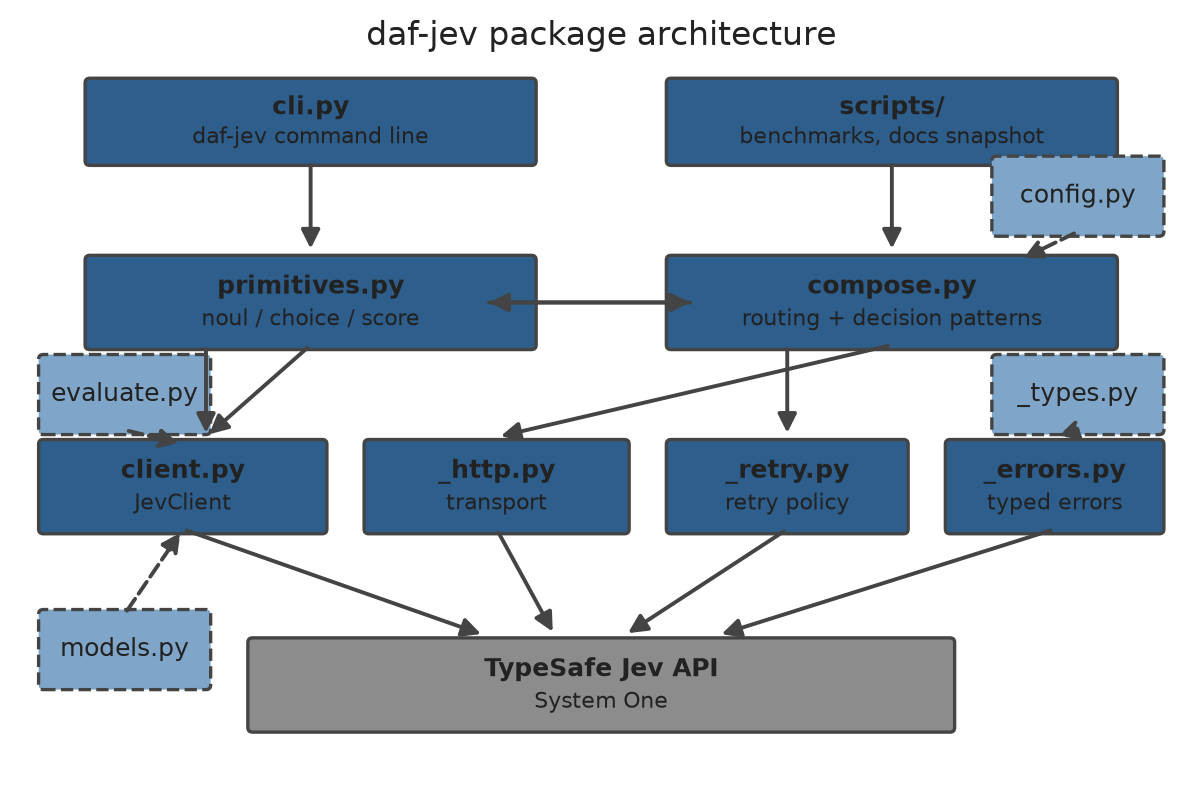
\includegraphics[width=0.85\linewidth,height=0.5\textheight,keepaspectratio,alt={Package layer diagram for daf-jev, drawn from the module graph of src/daf\_jev/. The application layer --- the CLI (src/daf\_jev/cli.py) and the thin orchestration scripts (scripts/, benchmarks/) --- delegates downward to the logic layer, where compose.py (pure decision patterns) and primitives.py (typed question builders and the QuestionSet container) sit over the wire dataclasses of \_types.py. client.py and \_http.py own the single transport to the System One endpoint, with \_retry.py providing the pure retry policy and \_errors.py the typed exception hierarchy; models.py and config.py enter as side inputs, and evaluate.py is the batch harness. The key structural takeaway is the enforced dependency direction: composition and primitives import no I/O machinery, so every decision pattern is testable against constructed answers without a network stand-in. Boxes are named modules only; no measured values appear in this schematic.}]{../figures/architecture.png}
\caption{Package layer diagram for daf-jev, drawn from the module graph
of \protect\texttt{src/daf\_jev/}. The application layer --- the CLI
(\protect\breaktt{src/daf\_jev/cli.py}) and the thin orchestration
scripts (\protect\texttt{scripts/}, \protect\texttt{benchmarks/}) ---
delegates downward to the logic layer, where \protect\texttt{compose.py}
(pure decision patterns) and \protect\texttt{primitives.py} (typed
question builders and the \protect\texttt{QuestionSet} container) sit
over the wire dataclasses of \protect\texttt{\_types.py}.
\protect\texttt{client.py} and \protect\texttt{\_http.py} own the single
transport to the System One endpoint, with \protect\texttt{\_retry.py}
providing the pure retry policy and \protect\texttt{\_errors.py} the
typed exception hierarchy; \protect\texttt{models.py} and
\protect\texttt{config.py} enter as side inputs, and
\protect\texttt{evaluate.py} is the batch harness. The key structural
takeaway is the enforced dependency direction: composition and
primitives import no I/O machinery, so every decision pattern is
testable against constructed answers without a network stand-in. Boxes
are named modules only; no measured values appear in this
schematic.}\label{fig:architecture}
\end{figure}

\subsection{Layered architecture}\label{layered-architecture}

The layers, bottom-up:

\begin{itemize}
\tightlist
\item
  \textbf{Transport} (\texttt{\_http.py}) --- a minimal
  \texttt{Transport} protocol with a synchronous and an asynchronous
  \texttt{httpx} implementation. It knows nothing about decisions; it
  posts JSON to a path and returns the raw response.
\item
  \textbf{Client} (\texttt{client.py}) --- \texttt{JevClient} /
  \texttt{AsyncJevClient} resolve the API key from the environment
  (injected mapping, process environment, then a \texttt{.env} file, in
  that precedence order via \texttt{config.py}), build the request for a
  state plus a mapping of questions, apply the retry policy, and map
  HTTP status classes onto the typed exception hierarchy of
  \texttt{\_errors.py}. The retry policy itself (\texttt{\_retry.py}) is
  a \emph{pure} function of the attempt number and an optional
  server-supplied retry hint --- exponential backoff with a base, a cap,
  and jitter, with the hint winning when present --- so its timing
  behavior is unit-testable without sleeping.
\item
  \textbf{Wire types} (\texttt{\_types.py}) --- frozen dataclasses for
  the three question types and the three answer types, a strict parser
  that rejects unknown answer shapes, a usage record, and the top-level
  response object with cached per-type views (\texttt{nouls},
  \texttt{choices}, \texttt{scores}).
\item
  \textbf{Primitives} (\texttt{primitives.py}) --- the ergonomic
  builders \texttt{noul()}, \texttt{choice()}, \texttt{score()} and the
  \texttt{QuestionSet} mapping container with additive composition
  (\texttt{add}, \texttt{merge}, \texttt{to\_wire}). No I/O.
\item
  \textbf{Composition} (\texttt{compose.py}) --- pure functions over
  answers, described below. No I/O; network access happens only through
  a client injected by the caller for multi-call helpers.
\item
  \textbf{Harness} (\texttt{evaluate.py}) --- the batch
  \texttt{Evaluator}, described below.
\end{itemize}

\subsection{Typed primitives}\label{typed-primitives}

\begin{figure}
\centering
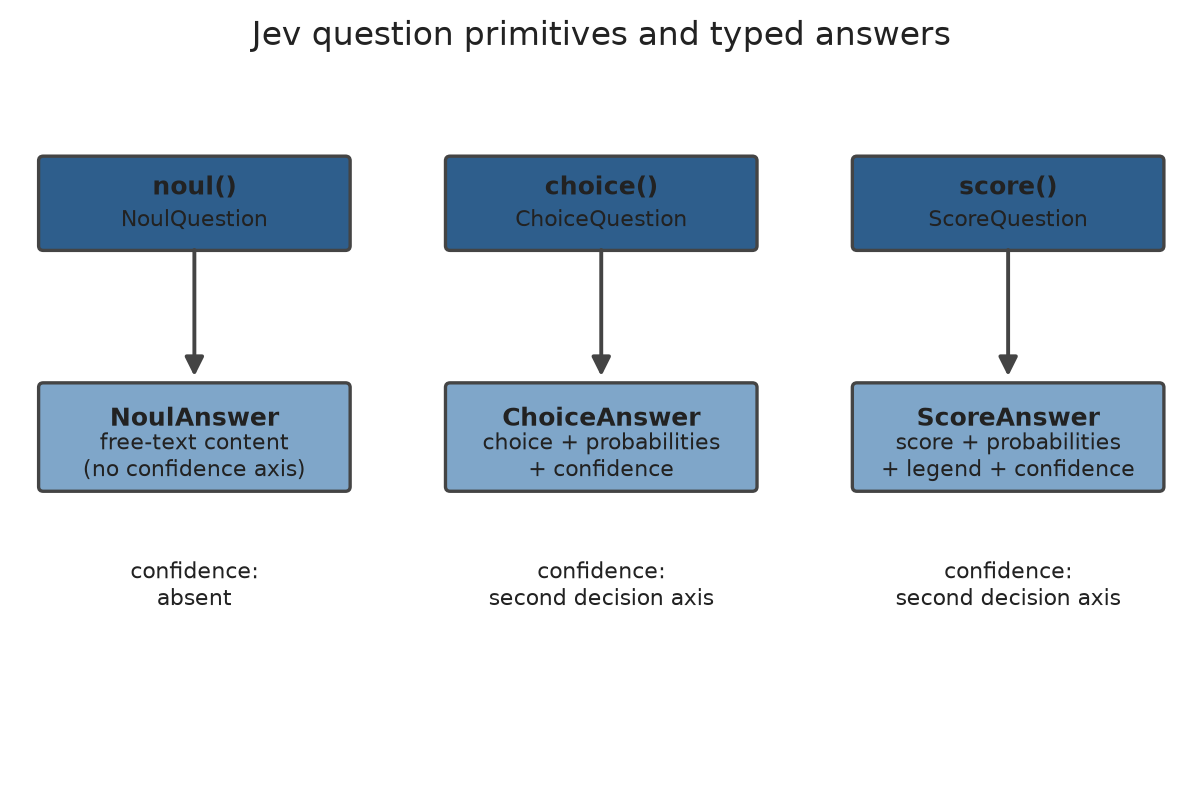
\includegraphics[width=0.85\linewidth,height=0.5\textheight,keepaspectratio,alt={The three question primitives of the System One surface and the typed answer shapes daf-jev parses them into, drawn as a schematic of the wire contract (sec.~). A noul question yields a calibrated yes/no probability; a choice question yields a selected label, a full probability distribution over the named options, and a scalar confidence; a score question yields a probability-weighted score over ordered levels together with the level legend, the level distribution, and a confidence. The takeaway is that the builders in primitives.py map one-to-one onto these shapes with strict, eager validation --- score criteria must carry at least two ordered levels, choice criteria must be non-empty, and the answer-side parser rejects any payload outside the discriminated union --- so downstream composition code can pattern-match on answers without defensive parsing. The diagram carries no measured data.}]{../figures/primitives_overview.png}
\caption{The three question primitives of the System One surface and the
typed answer shapes daf-jev parses them into, drawn as a schematic of
the wire contract (sec.~\ref{sec:jev_model}). A \protect\texttt{noul}
question yields a calibrated yes/no probability; a
\protect\texttt{choice} question yields a selected label, a full
probability distribution over the named options, and a scalar
confidence; a \protect\texttt{score} question yields a
probability-weighted score over ordered levels together with the level
legend, the level distribution, and a confidence. The takeaway is that
the builders in \protect\texttt{primitives.py} map one-to-one onto these
shapes with strict, eager validation --- score criteria must carry at
least two ordered levels, choice criteria must be non-empty, and the
answer-side parser rejects any payload outside the discriminated union
--- so downstream composition code can pattern-match on answers without
defensive parsing. The diagram carries no measured
data.}\label{fig:primitives}
\end{figure}

The builders in fig.~\ref{fig:primitives} map one-to-one onto the wire
contract of sec.~\ref{sec:jev_model}. Validation is strict and eager:
score criteria must carry at least two ordered levels, choice criteria
must be non-empty, and the answer-side parser rejects any payload whose
shape does not match the discriminated union exactly. The payoff of
strictness is that downstream composition code can pattern-match on
answers without defensive parsing --- the type system, not runtime
guesswork, guarantees the shapes.

\subsection{Composable decision
patterns}\label{composable-decision-patterns}

The composition layer implements the documented TypeSafe patterns as
pure functions \citep{typesafe2026patterns}:

\begin{itemize}
\tightlist
\item
  \textbf{\breaktt{composite\_score(answer,\ weights=None)}} --- the
  expected value of a \texttt{score} answer over its level indices,
  uniform by default or under caller-supplied weights (which must be
  finite and positive-massing). This turns an ordinal rating into a
  comparable scalar without a second model call.
\item
  \textbf{\breaktt{confidence\_gate(answer,\ threshold,\ below)}} ---
  returns the answer's primary value when its confidence meets the
  caller's threshold, and the \texttt{below} verdict otherwise. The
  threshold is owned by the calling code, never by the package.
\item
  \textbf{\breaktt{route(answer,\ handlers,\ min\_confidence,\ fallback)}}
  --- dispatches to the handler registered for a \texttt{choice}
  answer's label, gated on a minimum confidence with an optional
  fallback handler; \texttt{pick} fans the same dispatch across every
  answer in a mapping.
\end{itemize}

\textbf{Batching fan-out and the Evaluator.} Because the model evaluates
questions independently and in parallel (sec.~\ref{sec:jev_model}), the
cheapest correct strategy is to batch a fixed question set into one
call. The \texttt{Evaluator} in \texttt{evaluate.py} inverts the axis:
it holds the question set fixed and runs it over \emph{many states},
concurrently --- through a thread pool for the synchronous client or
\texttt{asyncio} with a semaphore for the asynchronous client. Per-state
failures never abort the batch; they are captured into the evaluation
record alongside the answers and the measured latency, so one malformed
state cannot cost the run. This harness is what the benchmark scripts in
sec.~\ref{sec:results} reuse for their fan-out measurements.

\textbf{Confidence-gated routing.} fig.~\ref{fig:confidence} illustrates
the three-band policy that \texttt{confidence\_gate} and \texttt{route}
implement: answers whose confidence clears the upper band are automated,
mid-band answers are routed to review, and answers below the lower band
are escalated. The boundary markers in the figure are \emph{example
thresholds} --- the semantics are the bands, not any particular cut
points, which remain policy owned by the caller.

\begin{figure}
\centering
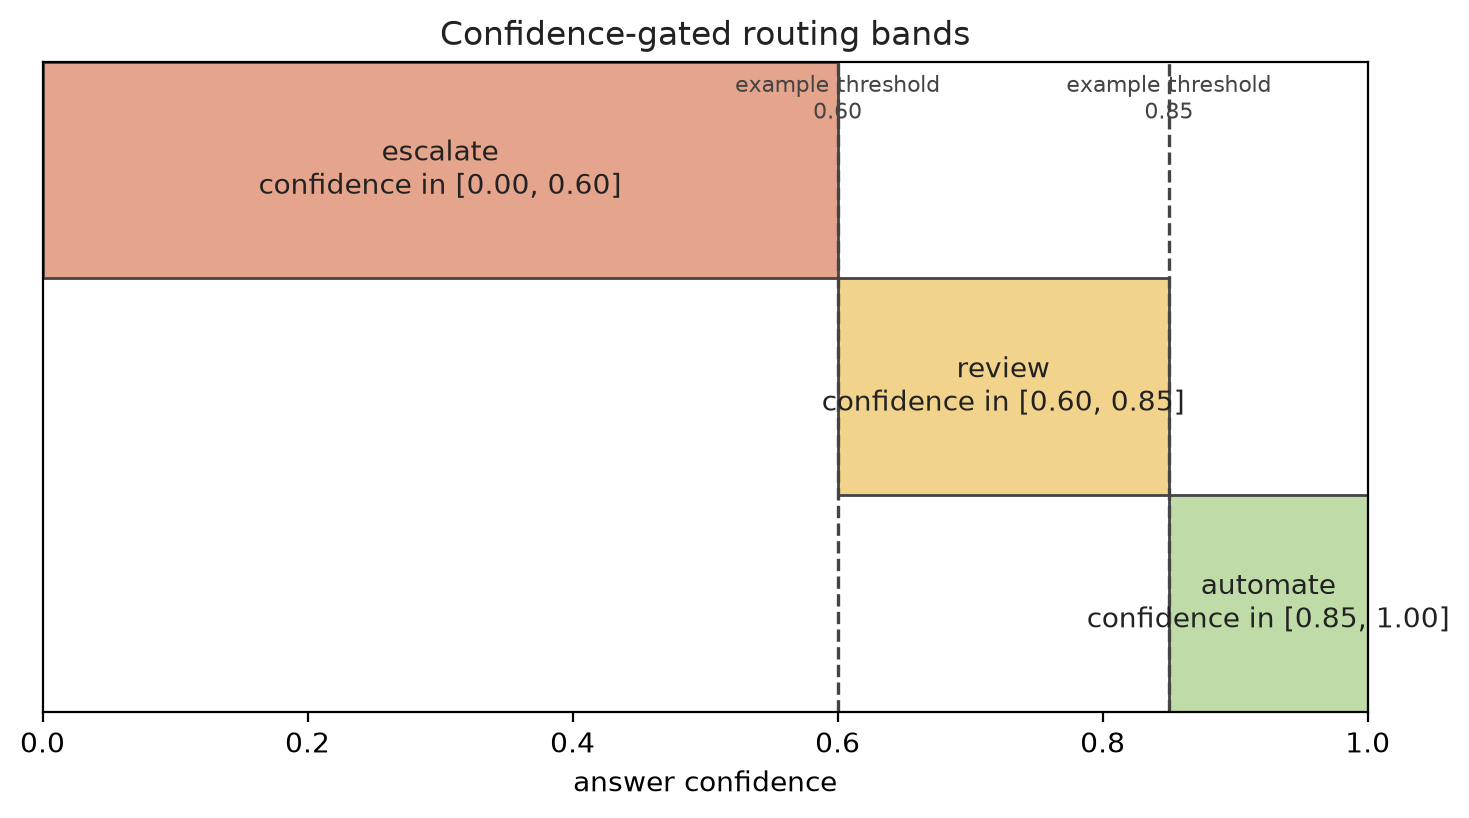
\includegraphics[width=0.8\linewidth,height=0.5\textheight,keepaspectratio,alt={Parametric illustration of confidence-gated routing as implemented by confidence\_gate() and route() in src/daf\_jev/compose.py (sec.~). The horizontal axis is the model-reported confidence on the unit interval; the three horizontal bands assign an action per confidence region --- automate above the upper boundary, route to review in the middle band, escalate below the lower boundary. The boundary markers are annotated as example thresholds: the semantics are the bands, not any particular cut points, and the actual thresholds remain policy owned by the caller. This figure is parametric and carries no measured data; sec.~ measures the latency and calibration properties that make running this policy inline sound.}]{../figures/confidence_bands.png}
\caption{Parametric illustration of confidence-gated routing as
implemented by \protect\breaktt{confidence\_gate()} and
\protect\texttt{route()} in \protect\breaktt{src/daf\_jev/compose.py}
(sec.~\ref{sec:methodology}). The horizontal axis is the model-reported
confidence on the unit interval; the three horizontal bands assign an
action per confidence region --- automate above the upper boundary,
route to review in the middle band, escalate below the lower boundary.
The boundary markers are annotated as example thresholds: the semantics
are the bands, not any particular cut points, and the actual thresholds
remain policy owned by the caller. This figure is parametric and carries
no measured data; sec.~\ref{sec:results} measures the latency and
calibration properties that make running this policy inline
sound.}\label{fig:confidence}
\end{figure}

\subsection{Design rulings}\label{design-rulings}

Four rulings shaped the codebase and are worth stating as contracts:

\begin{enumerate}
\def\labelenumi{\arabic{enumi}.}
\tightlist
\item
  \textbf{Pure logic, injected I/O.} Everything under
  \texttt{compose.py}, \texttt{primitives.py}, \texttt{\_types.py}, and
  \texttt{\_retry.py} performs no I/O; network access is confined to the
  transport and client layer and is injectable (clock, sleep, transport)
  for deterministic tests.
\item
  \textbf{Real stand-ins, no mocks.} The test suite drives the real HTTP
  transport against a real local HTTP server fixture rather than
  patching client internals, so retry, timeout, and error-mapping
  behavior is exercised end to end.
\item
  \textbf{Pure retry policy.} Backoff timing is a function of the
  attempt number and the server's retry hint alone --- testable without
  sleeping, and identical across the sync and async clients.
\item
  \textbf{Snapshotted documentation.} The bundled documentation snapshot
  carries a manifest of per-page content hashes and a snapshot
  identifier, and a CLI subcommand re-hashes the tree to detect drift
  (sec.~\ref{sec:reproducibility}). Prose claims about the model are
  therefore checkable against an immutable, verified source rather than
  a moving website.
\end{enumerate}

\newpage

\section{Integration Surfaces: CLI, MCP Server, Agent Skill, and Worked
Examples}\label{sec:integration_surfaces}

The Python API is the primary door into daf-jev, but not the only one.
Four additional surfaces sit on top of the same layering described in
sec.~\ref{sec:methodology} --- transport, client, primitives,
composition --- and add accessibility rather than logic: the
command-line interface, an MCP server, an agent skill, and a set of
runnable examples. Each one delegates to the very modules described
above and contains no decision code of its own. A behaviour fixed in the
composition layer therefore reaches every consumer at once: the CLI and
the MCP server call the same client and compose functions the Python API
calls, the skill documents those entry points, and the examples exercise
them.

\subsection{Command-line interface}\label{command-line-interface}

The \texttt{daf-jev} console script (\breaktt{src/daf\_jev/cli.py})
exposes five subcommands that cover the package's main paths without
writing Python:

\begin{itemize}
\tightlist
\item
  \textbf{\texttt{daf-jev\ ask}} --- one call, one state: the state
  arrives as inline text or JSON (\texttt{-\/-state}) or from a file
  (\texttt{-\/-state-file}), and one or more
  \texttt{-\/-question\ ID=SPEC} flags build the question set from a
  compact grammar (\texttt{noul:\textless{}instructions\textgreater{}},
  \texttt{choice:\textless{}instructions\textgreater{}:k1=desc,k2=...},
  \texttt{score:\textless{}instructions\textgreater{}:l1,l2,...}). The
  answer is emitted as JSON (compact by default, \texttt{-\/-pretty} for
  readability).
\item
  \textbf{\breaktt{daf-jev\ evaluate}} --- the batch \texttt{Evaluator}
  of sec.~\ref{sec:methodology} as a command: a fixed question set runs
  concurrently over many states, and the evaluation records --- answers,
  per-state failures, and measured latency --- are emitted as JSON.
\item
  \textbf{\texttt{daf-jev\ models}} --- lists the available model
  surface, with \texttt{-\/-pick\ latest|{}first|{}last}
  selecting a single identifier for scripting.
\item
  \textbf{\breaktt{daf-jev\ docs-verify}} --- re-hashes the bundled
  documentation snapshot against its manifest and exits non-zero on
  drift; this is the command-line face of Design ruling 4
  (sec.~\ref{sec:reproducibility}).
\item
  \textbf{\texttt{daf-jev\ serve}} --- launches the MCP server described
  next, over the stdio transport.
\end{itemize}

The CLI is a thin adapter in the same sense as the composition layer is
pure: it parses arguments, delegates to the client or the composition
helpers, and serializes the result. It owns no retry policy, no parsing
of answers, and no thresholds.

\subsection{MCP server}\label{mcp-server}

\breaktt{src/daf\_jev/mcp\_server.py} exposes the same core to any
MCP-capable agent host. Launched with \texttt{daf-jev\ serve} over the
stdio transport, it advertises seven tools that mirror the package
one-to-one:

\begin{itemize}
\tightlist
\item
  \texttt{jev\_ask} --- drives the client's single-call path: named
  questions (\texttt{noul} / \texttt{choice} / \texttt{score}, given in
  the same compact grammar the CLI accepts or as native
  \texttt{\{type,\ instructions,\ criteria\}} dicts) asked about one
  state;
\item
  \texttt{jev\_evaluate} --- drives the batch path, running a fixed
  question set over many states concurrently;
\item
  \texttt{jev\_models} --- reports (and optionally picks from) the
  available model surface;
\item
  \breaktt{jev\_composite\_score}, \breaktt{jev\_confidence\_gate}, and
  \texttt{jev\_tiered\_gate} --- expose the composition patterns of
  sec.~\ref{sec:methodology}; these combine answers locally with no API
  call at all;
\item
  \texttt{jev\_docs\_verify} --- re-runs the documentation drift check
  of Design ruling 4.
\end{itemize}

A \breaktt{jev://docs/snapshot} resource serves a summary of the bundled
documentation snapshot itself, so an agent can inspect what the
model-level claims rest on without leaving its host. The server is a
thin adapter --- it owns no retry policy, no parsing, and no thresholds;
every call delegates to \texttt{JevClient}, \texttt{AsyncJevClient}, or
the pure composition functions.

Registering the server with an MCP client is a one-block stdio
configuration; with the package installed (or, equivalently,
\texttt{command:\ "uv"} with
\texttt{args:\ {[}"run",\ "daf-jev",\ "serve"{]}} inside the
repository):

\begin{Shaded}
\begin{Highlighting}[]
\FunctionTok{\{}
  \DataTypeTok{"mcpServers"}\FunctionTok{:} \FunctionTok{\{}
    \DataTypeTok{"daf{-}jev"}\FunctionTok{:} \FunctionTok{\{}
      \DataTypeTok{"command"}\FunctionTok{:} \StringTok{"daf{-}jev"}\FunctionTok{,}
      \DataTypeTok{"args"}\FunctionTok{:} \OtherTok{[}\StringTok{"serve"}\OtherTok{]}
    \FunctionTok{\}}
  \FunctionTok{\}}
\FunctionTok{\}}
\end{Highlighting}
\end{Shaded}

The MCP extra (\texttt{pip\ install\ "daf-jev{[}mcp{]}"} or
\texttt{uv\ sync\ -\/-extra\ mcp}) is the only optional dependency this
surface adds; the core package does not depend on it.

\subsection{Agent skill}\label{agent-skill}

\breaktt{skills/daf-jev/SKILL.md} is a skill manifest for coding agents:
it states when to reach for the package, and how --- the builders and
their constraints, the client surface, the evaluation harness, the
composition patterns, the CLI subcommands, and the MCP tools --- so an
agent can use the package correctly without reading its source. The
skill carries no logic of its own; it is documentation positioned where
agents look for it, and it points at the same entry points the CLI and
MCP server expose.

\subsection{Worked examples}\label{worked-examples}

Four self-contained scripts under \texttt{examples/} walk the typical
integration path from a first call to a batch evaluation, doubling as
executable documentation of the composition layer:

\begin{itemize}
\tightlist
\item
  \textbf{\texttt{quickstart.py}} --- the shortest path to a typed
  answer: build a question set, make one call, read the typed answers;
\item
  \textbf{\breaktt{triage\_router.py}} --- confidence-gated routing end
  to end: a \texttt{choice} call dispatched by \texttt{route()} with a
  fallback for low-confidence answers;
\item
  \textbf{\breaktt{composite\_scoring.py}} --- a \texttt{score} call
  turned into a comparable scalar by \breaktt{composite\_score()} and
  verdict-banded by \breaktt{confidence\_gate()};
\item
  \textbf{\breaktt{evaluate\_corpus.py}} --- the batch \texttt{Evaluator}
  over many states, with per-state failure capture and summary
  aggregates.
\end{itemize}

Each script runs against the real endpoint when an API key is present
and prints a clear skip notice otherwise, matching the benchmark
convention of sec.~\ref{sec:experimental_setup}.

\newpage

\section{Results: Batching Economics, Pipeline Latency, and Confidence
Calibration under Live-API Load}\label{sec:results}

This section reports the three live-API benchmarks that quantify the
design claims of sec.~\ref{sec:methodology}: the batching benchmark,
which reproduces the documented parallel-questions pattern
\citep{typesafe2026patterns}, the decision-pattern latency benchmark,
and the self-consistency calibration benchmark. All run against the real
jev-latest model; every value below is injected from the benchmark
outputs at render time, and the figures are regenerated from the same
JSON files, so prose, tables, and figures share one source of truth. The
batching and latency results reported here were recorded on 2026-09-16;
the calibration results on 2026-09-16.

\subsection{Batching speedup and token
cost}\label{batching-speedup-and-token-cost}

The batching benchmark compares two strategies over the same state and
question mix: one call carrying all questions in a batch, versus one
sequential single-question call per question, repeated for each
configured batch width over multiple measured runs. The answers are
unchanged by batching (the parallel-sampler semantics of
sec.~\ref{sec:jev_model}); what changes is wall time --- a single round
trip versus one round trip per question --- and token cost, because the
sequential strategy re-sends the state once per question.

fig.~\ref{fig:batching} shows the measured speedup per batch width
together with the token-cost ratio on a secondary axis.

\begin{figure}
\centering
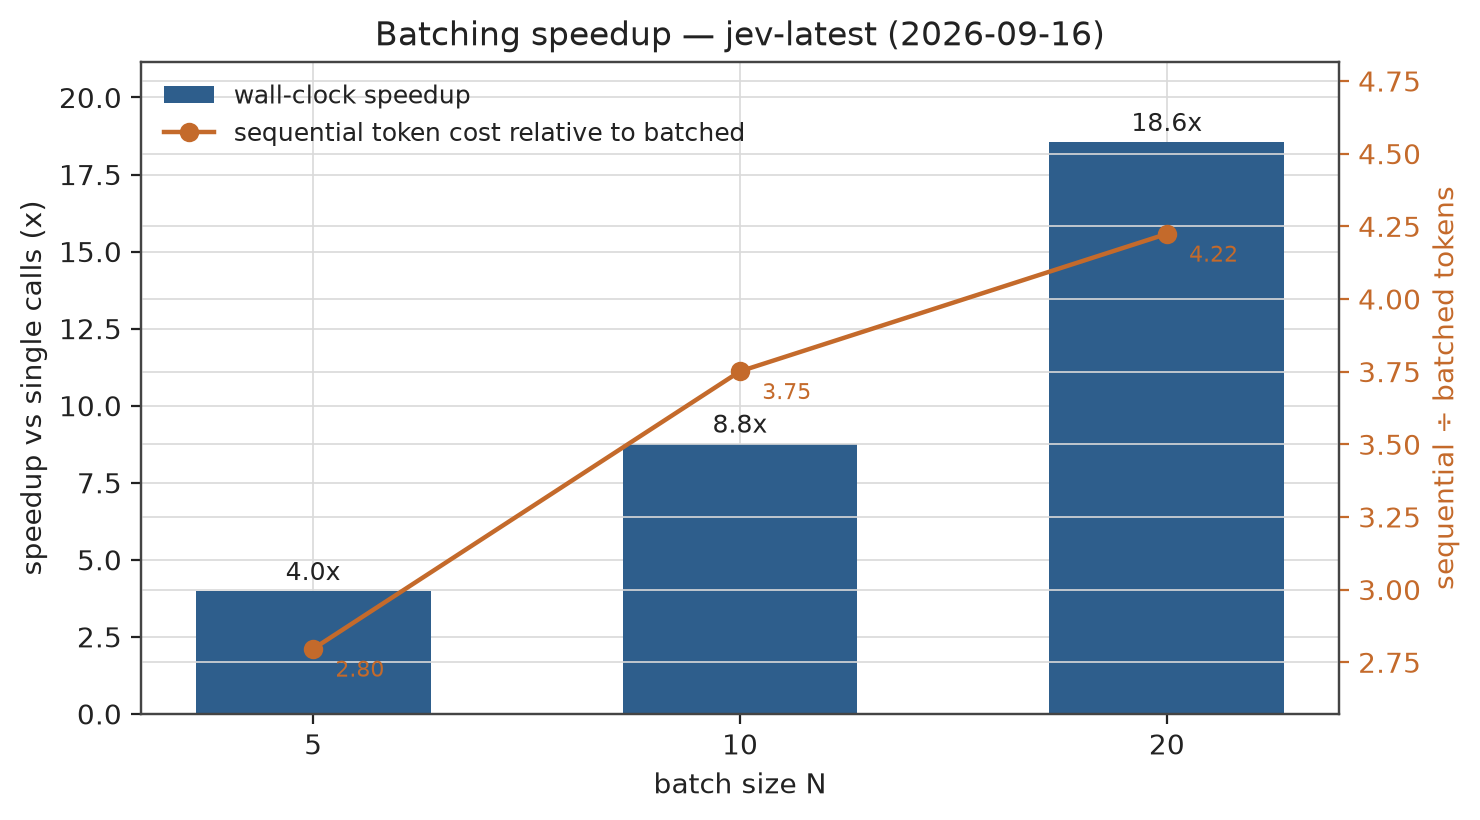
\includegraphics[width=0.85\linewidth,height=0.5\textheight,keepaspectratio,alt={Batching speedup of the jev-latest model versus sequential single-question calls, measured by benchmarks/bench\_batching.py on 2026-09-16 against the live API. Bars give the wall-time speedup of one batched call over one sequential call per question for each configured batch width (5, 10, and 20 questions per batch, tabulated in tbl.~); the secondary axis traces the token-cost ratio --- sequential tokens divided by batched tokens --- which rises above unity because the sequential strategy re-sends the state paragraph once per question. Each bar is annotated with its measured value, and the rendered title carries the model identifier and run date read from the benchmark JSON itself. The takeaway: the speedup grows with batch width as the fixed per-call overhead amortizes, while the batched strategy is simultaneously cheaper in tokens, not only faster.}]{../figures/batching_speedup.png}
\caption{Batching speedup of the jev-latest model versus sequential
single-question calls, measured by
\protect\breaktt{benchmarks/bench\_batching.py} on 2026-09-16 against the
live API. Bars give the wall-time speedup of one batched call over one
sequential call per question for each configured batch width (5, 10, and
20 questions per batch, tabulated in tbl.~\ref{tbl:batching}); the
secondary axis traces the token-cost ratio --- sequential tokens divided
by batched tokens --- which rises above unity because the sequential
strategy re-sends the state paragraph once per question. Each bar is
annotated with its measured value, and the rendered title carries the
model identifier and run date read from the benchmark JSON itself. The
takeaway: the speedup grows with batch width as the fixed per-call
overhead amortizes, while the batched strategy is simultaneously cheaper
in tokens, not only faster.}\label{fig:batching}
\end{figure}

tbl.~\ref{tbl:batching} tabulates the measured speedups. The speedup
grows with batch width, as expected from the round-trip accounting: the
fixed per-call overhead is amortized over more questions, and the state
is transmitted once rather than once per question.

\begin{longtable}[]{@{}ll@{}}
\caption{Wall-time speedup of one batched call versus one sequential
call per question, per configured batch width, recorded by
\protect\breaktt{benchmarks/bench\_batching.py} against the jev-latest
model on 2026-09-16. Values are injected from the benchmark JSON at
render time.}\label{tbl:batching}\tabularnewline
\toprule\noalign{}
Questions per batch & Wall-time speedup vs sequential \\
\midrule\noalign{}
\endfirsthead
\toprule\noalign{}
Questions per batch & Wall-time speedup vs sequential \\
\midrule\noalign{}
\endhead
\bottomrule\noalign{}
\endlastfoot
5 & 3.98 \\
10 & 8.77 \\
20 & 18.55 \\
\end{longtable}

Token cost moves in the same direction. The recorded
\breaktt{token\_cost\_ratio} expresses the sequential strategy's token
consumption relative to the batched strategy's: at the widest configured
batch width the sequential strategy consumes 4.22 times the tokens of
the batched call. The state paragraph dominates the input tokens of a
single-question call, so re-sending it per question makes the sequential
strategy strictly more expensive in addition to being slower.

\subsection{Decision-pipeline latency}\label{decision-pipeline-latency}

The second benchmark measures end-to-end latency of two composition
pipelines --- the network call plus the local composition logic, exactly
as an application would run them:

\begin{itemize}
\tightlist
\item
  \textbf{composite\_score} --- one \texttt{score} call, then
  \texttt{composite\_score} over the answer, then a
  \texttt{confidence\_gate} verdict;
\item
  \textbf{intent\_routing} --- one \texttt{choice} call, then
  \texttt{route()} dispatching to a trivial handler.
\end{itemize}

Each pipeline is executed 6 times; tbl.~\ref{tbl:latency} reports the
median (p50) and tail (p95) wall times per pipeline, and
fig.~\ref{fig:latency} plots them side by side.

\begin{figure}
\centering
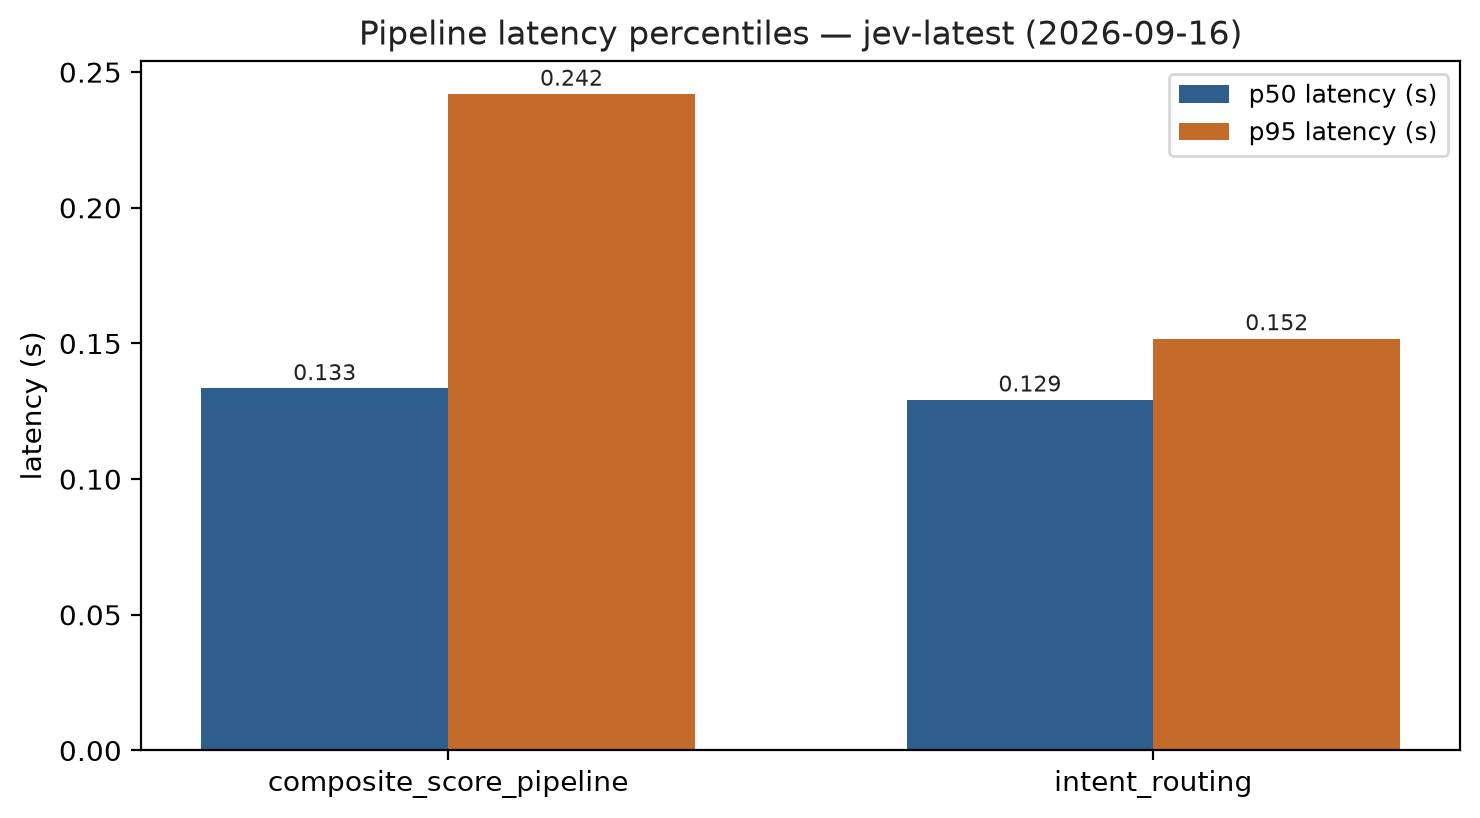
\includegraphics[width=0.85\linewidth,height=0.5\textheight,keepaspectratio,alt={Median (p50) and tail (p95) end-to-end wall time per decision pipeline, measured by benchmarks/bench\_patterns.py over 6 runs against the jev-latest model on 2026-09-16. Each pipeline group --- composite scoring (one score call, then composite\_score and a confidence\_gate verdict) and intent routing (one choice call, then route() dispatch) --- shows paired p50/p95 bars covering the full network round trip plus the local composition logic; values are tabulated in tbl.~ and read from the benchmark JSON fields at figure-generation time. The takeaway: both pipelines sit within the model's millisecond-scale latency envelope, so the pure-logic composition layer adds no measurable latency beyond the network round trip and the gating policy can run inline on interactive request paths.}]{../figures/latency_percentiles.png}
\caption{Median (p50) and tail (p95) end-to-end wall time per decision
pipeline, measured by \protect\breaktt{benchmarks/bench\_patterns.py}
over 6 runs against the jev-latest model on 2026-09-16. Each pipeline
group --- composite scoring (one \protect\texttt{score} call, then
\protect\texttt{composite\_score} and a
\protect\texttt{confidence\_gate} verdict) and intent routing (one
\protect\texttt{choice} call, then \protect\texttt{route()} dispatch)
--- shows paired p50/p95 bars covering the full network round trip plus
the local composition logic; values are tabulated in
tbl.~\ref{tbl:latency} and read from the benchmark JSON fields at
figure-generation time. The takeaway: both pipelines sit within the
model's millisecond-scale latency envelope, so the pure-logic
composition layer adds no measurable latency beyond the network round
trip and the gating policy can run inline on interactive request
paths.}\label{fig:latency}
\end{figure}

\begin{longtable}[]{@{}
  >{\raggedright\arraybackslash}p{(\linewidth - 4\tabcolsep) * \real{0.2778}}
  >{\raggedright\arraybackslash}p{(\linewidth - 4\tabcolsep) * \real{0.3750}}
  >{\raggedright\arraybackslash}p{(\linewidth - 4\tabcolsep) * \real{0.3472}}@{}}
\caption{End-to-end wall time (network round trip plus local composition
logic) per decision pipeline, median and tail over 6 runs recorded by
\protect\breaktt{benchmarks/bench\_patterns.py} against the jev-latest
model on 2026-09-16. Values are injected from the benchmark JSON at
render time.}\label{tbl:latency}\tabularnewline
\toprule\noalign{}
\begin{minipage}[b]{\linewidth}\raggedright
Pipeline
\end{minipage} & \begin{minipage}[b]{\linewidth}\raggedright
Median wall time, p50 (s)
\end{minipage} & \begin{minipage}[b]{\linewidth}\raggedright
Tail wall time, p95 (s)
\end{minipage} \\
\midrule\noalign{}
\endfirsthead
\toprule\noalign{}
\begin{minipage}[b]{\linewidth}\raggedright
Pipeline
\end{minipage} & \begin{minipage}[b]{\linewidth}\raggedright
Median wall time, p50 (s)
\end{minipage} & \begin{minipage}[b]{\linewidth}\raggedright
Tail wall time, p95 (s)
\end{minipage} \\
\midrule\noalign{}
\endhead
\bottomrule\noalign{}
\endlastfoot
composite\_score & 0.133 & 0.242 \\
intent\_routing & 0.129 & 0.152 \\
\end{longtable}

\subsection{Calibration}\label{calibration}

Latency says nothing about whether the composed decisions are
trustworthy, so the third benchmark measures how far the model's
reported confidence tracks its own agreement behaviour.
\breaktt{benchmarks/bench\_calibration.py} runs 6 short states 5 times
each against the jev-latest model and scores choice answers under a
\emph{self-consistency proxy}: a sample counts as correct when it agrees
with the modal choice across the repeats of the same state. Because a
yes/no probability carries no per-sample label to agree with, noul
answers are scored for repeat-to-repeat stability instead, via the mean
absolute gap between every pair of repeated answers. No external ground
truth is consulted anywhere in this benchmark --- the correctness proxy
is self-agreement, not verified outcomes.

tbl.~\ref{tbl:calibration} reports the aggregate scores over the run,
and fig.~\ref{fig:calibration} plots the reliability curve per
confidence bucket.

\begin{longtable}[]{@{}ll@{}}
\caption{Calibration summary over 6 states \texorpdfstring{\ensuremath{\times}}{x} 5 repeats recorded by
\protect\breaktt{benchmarks/bench\_calibration.py} against the jev-latest
model on 2026-09-16. Choice correctness is a self-consistency proxy ---
agreement with the modal choice across repeats --- not accuracy against
ground truth; the mean pairwise noul gap measures repeat-to-repeat
answer stability rather than correctness. Values are injected from the
benchmark JSON at render time.}\label{tbl:calibration}\tabularnewline
\toprule\noalign{}
Metric & Value \\
\midrule\noalign{}
\endfirsthead
\toprule\noalign{}
Metric & Value \\
\midrule\noalign{}
\endhead
\bottomrule\noalign{}
\endlastfoot
Expected calibration error (choice, proxy) & 0.0730 \\
Brier score (choice, proxy) & 0.0252 \\
Mean pairwise noul gap & 0.0050 \\
\end{longtable}

\begin{figure}
\centering
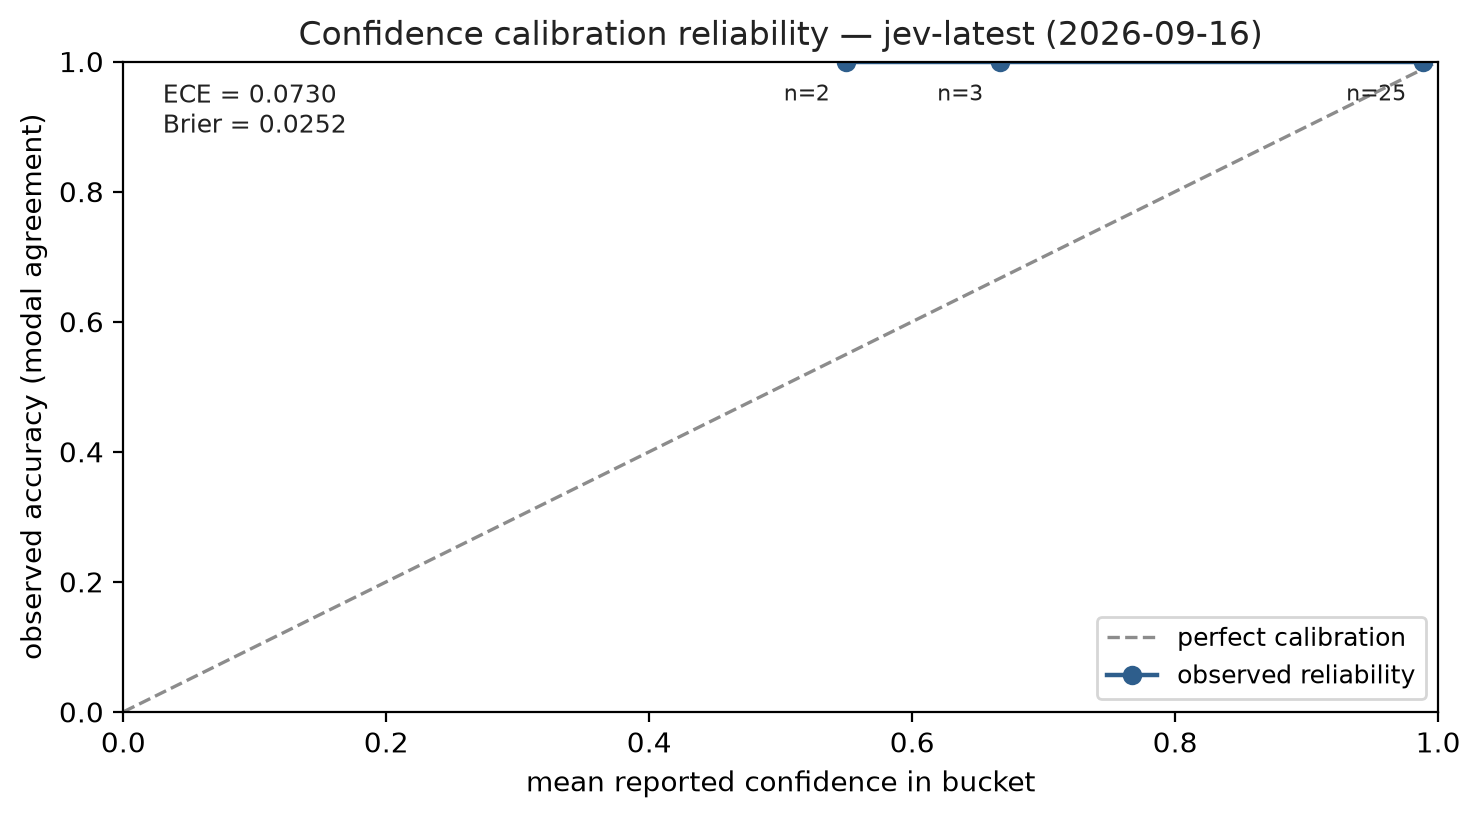
\includegraphics[width=0.85\linewidth,height=0.5\textheight,keepaspectratio,alt={Reliability diagram of choice-answer confidence under the self-consistency proxy, measured by benchmarks/bench\_calibration.py over 6 states \texorpdfstring{\ensuremath{\times}}{x} 5 repeats against the jev-latest model on 2026-09-16. Each point is a confidence bucket plotting mean reported confidence against proxy accuracy, where proxy accuracy is agreement with the modal choice across repeats of the same state; the dashed diagonal marks perfect agreement between stated confidence and observed proxy accuracy. Because the proxy scores self-agreement rather than verified correctness, proximity to the diagonal indicates consistency between stated confidence and repeat-stable behaviour --- not truthfulness about the world. Aggregate scores are tabulated in tbl.~.}]{../figures/calibration_reliability.png}
\caption{Reliability diagram of choice-answer confidence under the
self-consistency proxy, measured by
\protect\breaktt{benchmarks/bench\_calibration.py} over 6 states \texorpdfstring{\ensuremath{\times}}{x} 5
repeats against the jev-latest model on 2026-09-16. Each point is a
confidence bucket plotting mean reported confidence against proxy
accuracy, where proxy accuracy is agreement with the modal choice across
repeats of the same state; the dashed diagonal marks perfect agreement
between stated confidence and observed proxy accuracy. Because the proxy
scores self-agreement rather than verified correctness, proximity to the
diagonal indicates consistency between stated confidence and
repeat-stable behaviour --- not truthfulness about the world. Aggregate
scores are tabulated in
tbl.~\ref{tbl:calibration}.}\label{fig:calibration}
\end{figure}

The expected calibration error of 0.0730 and the Brier score of 0.0252
indicate that reported choice confidence is broadly consistent with the
proxy labels, and the mean pairwise noul gap of 0.0050 shows that
repeated noul answers on the same state are nearly identical. These
claims extend exactly as far as the proxy does. Self-consistency can
establish that the model is stable across repeats and that its
confidence ordering is internally coherent; it cannot certify that the
answers are correct about the world, because the proxy labels are
generated by the same model whose calibration is being measured. The
benchmark is therefore evidence of calibrated, repeatable decision
behaviour under a reproducible proxy --- a necessary, not sufficient,
condition for deploying these gates on real decisions.

\subsection{Interpretation}\label{interpretation}

Four observations tie the measurements back to the design rulings of
sec.~\ref{sec:methodology}. First, the batching speedups in
tbl.~\ref{tbl:batching} confirm that the parallel-sampler semantics
translate directly into wall-clock savings: the batched strategy is
faster at every configured width, and the gap widens with width exactly
as the round-trip accounting predicts. Second, the token-cost ratio
above unity at the widest width --- the sequential strategy's token
consumption relative to the batched call's --- shows that batching is
not merely faster but cheaper, because the state is transmitted once ---
so the pattern documented in the primary source
\citep{typesafe2026patterns} holds end to end for a third-party client
implementation. Third, the pipeline latencies in tbl.~\ref{tbl:latency}
sit within the model's millisecond-scale latency envelope
(sec.~\ref{sec:jev_model}): the pure-logic composition layer adds no
measurable latency beyond the network round trip, which is precisely
what allows confidence-gated routing to run inline on interactive
request paths rather than in a background queue. Fourth, the calibration
summary in tbl.~\ref{tbl:calibration} supports the calibrated-decision
premise of the confidence-gated patterns described in
sec.~\ref{sec:methodology} --- reported choice confidence aligns with
repeat-stable behaviour, and noul answers are stable across repeats ---
under the self-consistency proxy semantics stated in the Calibration
section, and only as far as those semantics extend.

\newpage

\section{Experimental Setup: Live-API Benchmark Protocol, Environment,
and Data Provenance}\label{sec:experimental_setup}

This section records the environment, configuration, and measurement
protocol behind the results in sec.~\ref{sec:results}, so that the runs
can be reproduced bit-for-bit in intent.

\subsection{Software environment}\label{software-environment}

All measurements were taken with daf-jev version 0.3.0, running under
3.14.6 on the platform reported as
\breaktt{macOS-26.6.2-arm64-arm-64bit-Mach-O}. The package targets Python
3.10 or newer and depends, at runtime, only on \texttt{httpx} for
transport and \texttt{pyyaml} for configuration parsing; the benchmark
scripts additionally use the standard library. The development toolchain
is \texttt{uv}-managed, and the unit test suite is executed with
\texttt{pytest} under a coverage gate.

The model-level claims in sec.~\ref{sec:jev_model} are grounded in a
local, hash-manifested snapshot of the TypeSafe documentation (snapshot
b79c9cd6008489f1, 108 pages) rather than the live website, so the
primary-source basis of this manuscript is itself versioned and
verifiable.

\subsection{Benchmark configuration}\label{benchmark-configuration}

All benchmarks execute against the real jev-latest model with a live API
key resolved through the package's credential precedence chain (injected
mapping, then process environment, then the project \texttt{.env} file).
Without a key, the scripts print a skip notice and exit successfully ---
they are benchmarks, not tests, and never run inside the test suite.

\begin{itemize}
\tightlist
\item
  \textbf{Batching benchmark} (\breaktt{benchmarks/bench\_batching.py})
  --- for each configured batch width (5, 10, 20 questions, as recorded
  under \breaktt{experiment.batching\_n\_values} in
  \breaktt{manuscript/config.yaml}), it compares one batched call against
  the same number of sequential single-question calls over a fixed state
  paragraph and a mixed noul/choice/score question set, repeating each
  strategy for the configured number of runs and recording wall time and
  token totals to
  \texttt{output/benchmarks/batching\_\textless{}date\textgreater{}.json}.
\item
  \textbf{Decision-pattern benchmark}
  (\breaktt{benchmarks/bench\_patterns.py}) --- runs the composite-score
  and intent-routing pipelines 6 times each (default recorded under
  \breaktt{experiment.patterns\_runs}), reporting mean, median, and tail
  wall times plus token totals to
  \texttt{output/benchmarks/patterns\_\textless{}date\textgreater{}.json}.
  An asynchronous mode executes the same runs concurrently through
  \texttt{AsyncJevClient} and compares against the sequential wall time.
\item
  \textbf{Calibration benchmark}
  (\breaktt{benchmarks/bench\_calibration.py}) --- runs 6 short states 5
  times each against the jev-latest model, scores choice answers under
  the self-consistency proxy (agreement with the modal choice across
  repeats) and noul answers by mean pairwise stability, and writes the
  expected calibration error, Brier score, per-bucket reliability data,
  and the mean pairwise noul gap to
  \texttt{output/benchmarks/calibration\_\textless{}date\textgreater{}.json},
  together with a \texttt{notes} field stating the proxy semantics.
\end{itemize}

All benchmark scripts take \texttt{-\/-runs} and \texttt{-\/-model}
arguments; the defaults are recorded as data under the
\texttt{experiment:} block of \breaktt{manuscript/config.yaml}, which is
the same file the manuscript-variable generator reads --- configuration,
prose, and figures cannot disagree about the protocol.

\subsection{Measurement protocol}\label{measurement-protocol}

Percentiles follow the benchmark helper shared by both scripts: the
reported tail statistic is the value at the ceiling-rank position of the
ordered sample, computed over the recorded runs rather than a sliding
window. Wall time covers the full pipeline --- transport, retries (none
should occur in a healthy run), parsing, and composition logic --- so
the numbers in tbl.~\ref{tbl:latency} are conservative upper bounds on
what an integrating application would add to its request path. Token
totals are read from the response usage records, not estimated.

This manuscript was generated at 2026-09-17T17:07:41Z; the rendered
values in sec.~\ref{sec:results} correspond to the benchmark JSONs
current at that timestamp, and the figure generators resolve ``latest''
the same way (latest by filename date) so that re-rendering after a new
benchmark run updates prose, tables, and figures together.

\newpage

\section{Reproducibility: Hashed Snapshots, Figure Registry, and
Machine-Checked Provenance}\label{sec:reproducibility}

Every artifact behind this manuscript --- figures, tables, token values,
and the documentation snapshot the model claims rest on --- is
regenerable from the repository with the commands below, and every
generated value reaches the prose through the token pipeline rather than
hand transcription.

\subsection{Artifact inventory and
hashing}\label{artifact-inventory-and-hashing}

\begin{itemize}
\item
  \textbf{Figures.} The seven figures of this manuscript are generated
  into \texttt{../figures/} by \breaktt{src/daf\_jev/figures.py} (one
  \texttt{generate\_\textless{}name\textgreater{}()} function per figure
  plus \breaktt{generate\_all(out\_dir)}), orchestrated by
  \breaktt{scripts/generate\_figures.py}:

\begin{Shaded}
\begin{Highlighting}[]
\ExtensionTok{uv}\NormalTok{ run python scripts/generate\_figures.py            }\CommentTok{\# all figures}
\ExtensionTok{uv}\NormalTok{ run python scripts/generate\_figures.py }\AttributeTok{{-}{-}only}\NormalTok{ batching\_speedup}
\end{Highlighting}
\end{Shaded}

  The data-driven figures read
  \breaktt{output/benchmarks/batching\_*.json},
  \breaktt{output/benchmarks/patterns\_*.json}, and
  \breaktt{output/benchmarks/calibration\_*.json}, resolving ``latest''
  by filename date; a missing benchmark file is reported as a clear
  error naming the missing file rather than silently producing an empty
  chart. The same rule applies to the graphical abstract of
  sec.~\ref{sec:abstract}, which composes the latest batching, latency,
  and calibration payloads into its live-outputs panel. The two
  schematic figures and the parametric confidence-band illustration
  require no data and no network.
\item
  \textbf{Figure registry.} Every figure is recorded in
  \breaktt{../figures/figure\_registry.json} --- seven entries, one per
  figure, each mapping the manuscript's cross-reference label
  (\breaktt{fig:graphical\_abstract} plus \breaktt{fig:architecture}
  through \texttt{fig:calibration}) to its filename, caption, section,
  and layout width --- so the figure set itself is a versioned data
  artifact rather than a convention.
\item
  \textbf{Calibration benchmark payloads.} The calibration run writes
  \texttt{output/benchmarks/calibration\_\textless{}date\textgreater{}.json}
  (per-bucket reliability data, expected calibration error, Brier score,
  the mean pairwise noul gap, and a \texttt{notes} field stating the
  self-consistency proxy semantics);
  \breaktt{benchmarks/bench\_calibration.py} regenerates it live, and the
  reliability figure \breaktt{../figures/calibration\_reliability.png} is
  rendered from the same payload by \breaktt{generate\_calibration()} in
  \breaktt{src/daf\_jev/figures.py}.
\item
  \textbf{Manuscript variables.} All dynamic values reach the prose as
  double-brace token placeholders, computed by
  \breaktt{src/daf\_jev/manuscript\_variables.py::generate\_variables(project\_root)}
  and written to \breaktt{output/data/manuscript\_variables.json} by the
  thin orchestrator
  \breaktt{scripts/z\_generate\_manuscript\_variables.py}, which then
  renders substituted copies of every section into
  \breaktt{output/manuscript/}. Running in strict mode fails if analysis
  outputs are missing; the \texttt{-\/-allow-draft} flag substitutes
  draft sentinels instead of failing, for early-stage renders only.
\item
  \textbf{Documentation snapshot.} The bundled snapshot of the TypeSafe
  documentation comprises 108 pages (1014.8 KiB) under
  \texttt{docs/reference/}, scraped on 2026-09-16 and identified as
  snapshot b79c9cd6008489f1. The manifest records a content hash per
  page plus the snapshot identifier; drift is detectable at any time
  with:

\begin{Shaded}
\begin{Highlighting}[]
\ExtensionTok{uv}\NormalTok{ run daf{-}jev docs{-}verify                 }\CommentTok{\# re{-}hash the tree, exit non{-}zero on drift}
\ExtensionTok{uv}\NormalTok{ run python scripts/scrape\_docs.py }\AttributeTok{{-}{-}check}   \CommentTok{\# same check without rewriting}
\end{Highlighting}
\end{Shaded}
\end{itemize}

\subsection{Test suite and coverage}\label{test-suite-and-coverage}

The test suite follows the no-mock convention: unit tests drive the real
transport against a real local HTTP server fixture, and live tests hit
the real API only when a key is present in the environment (they skip
with a notice otherwise). The suite comprises 17 test files --- 260 unit
tests and 2 live tests --- collected with:

\begin{Shaded}
\begin{Highlighting}[]
\ExtensionTok{uv}\NormalTok{ run pytest tests/unit }\AttributeTok{{-}{-}cov}\OperatorTok{=}\NormalTok{src     }\CommentTok{\# unit suite under the coverage gate}
\VariableTok{JEV\_API\_KEY}\OperatorTok{=}\NormalTok{... }\ExtensionTok{uv}\NormalTok{ run pytest tests/live   }\CommentTok{\# live tests against the real API}
\end{Highlighting}
\end{Shaded}

Measured coverage over the package source stands at 91.73, enforced by
the coverage gate configured in \texttt{pyproject.toml}. Test and
collection counts are computed at variable-generation time by collecting
the suite; if collection is unavailable in a given environment, the
corresponding values are reported as draft sentinels rather than
fabricated.

\subsection{Provenance chain}\label{provenance-chain}

The certification chain is: benchmark scripts write dated JSON payloads
\texorpdfstring{\ensuremath{\to}}{->} figure generators read those payloads and render
\breaktt{../figures/*.png} \texorpdfstring{\ensuremath{\to}}{->} the variable generator reads the same
payloads plus \breaktt{manuscript/config.yaml}, \texttt{pyproject.toml},
the test suite, and the docs manifest to compute the token mapping \texorpdfstring{\ensuremath{\to}}{->} the
injection step substitutes tokens into \breaktt{output/manuscript/*.md} \texorpdfstring{\ensuremath{\to}}{->}
the renderer consumes the substituted copies. No numeric fact in this
paper has a hand-maintained copy; the environment of record is
\breaktt{macOS-26.6.2-arm64-arm-64bit-Mach-O} under 3.14.6, and the
rendered edition is version 0.3.0 of this manuscript, generated at
2026-09-17T17:07:41Z.

\newpage

\section{Scope, Limitations, and Related Work: Early-Access Model, Proxy
Metrics, and the Structured-Decision Landscape}\label{sec:scope}

\subsection{Scope and limitations}\label{scope-and-limitations}

This manuscript describes an early, rapidly evolving package, and four
caveats bound every claim in it.

\textbf{Single-model measurements.} All benchmarks in
sec.~\ref{sec:results} were recorded against the jev-latest model at the
configuration described in sec.~\ref{sec:experimental_setup}. The
package accepts a per-call model override, but nothing here
characterizes how the speedups, token ratios, or latency percentiles
transfer across models or across provider-side changes to the same
model; re-running the two benchmark scripts against another setting is
the intended way to extend the measurements, and the render-time token
pipeline picks up the new payloads automatically.

\textbf{Live-API variance.} The measurements are wall-clock observations
of a shared remote service. Run-to-run variation from network conditions
and provider load is inherent; the percentile protocol in
sec.~\ref{sec:experimental_setup} reports medians and tails rather than
single samples, but the values should be read as representative of a
healthy session, not as service-level guarantees.

\textbf{Early-access documentation basis.} The model-level claims in
sec.~\ref{sec:jev_model} rest on a hash-manifested snapshot of the
vendor's documentation (snapshot b79c9cd6008489f1) rather than on the
vendor's release process. The package documents an early-access surface:
wire shapes, model identifiers, and documented patterns can change
upstream, and the \texttt{docs-verify} command plus a re-scrape
(sec.~\ref{sec:reproducibility}) is the mechanism for detecting and
absorbing such changes. Behavior not covered by the snapshot is
implemented as a stated assumption rather than a verified fact.

\textbf{Early-release status.} The package is published for
reproducibility and reuse --- the source is versioned, MIT-licensed, and
mirrored in a public repository, and this manuscript's edition carries a
versioned archival deposit alongside it --- but it remains an early
release of a tool built against an early-access model surface. The DOI
of record identifies the concept of this deposit; individual editions
are versioned beneath it, and the caveats above travel with every
edition.

\subsection{Related work}\label{related-work}

\textbf{Structured output from generative LLMs.} The mainstream approach
to software-consumable model answers is constrained decoding:
JSON-schema-constrained generation, function calling, and post-hoc
validators over generated text. These techniques constrain the
\emph{syntax} of free-text generation but inherit its semantics --- a
well-formed JSON payload can still encode an overconfident or
miscalibrated judgment, and nothing in the decoding contract expresses
uncertainty as calibrated probability. The decision-model approach of
sec.~\ref{sec:jev_model} differs at the training level: RLCD optimizes
for decisions and calibrated probabilities as the output contract itself
\citep{typesafe2026systemoneconcept}, rather than for text that a schema
hopes to bound.

\textbf{RLHF versus RLCD.} RLHF and its verifiable-reward variants adapt
a pretrained model by optimizing text quality against human preferences
or checkable rewards. RLCD instead optimizes a different output contract
--- decisions with calibrated probability distributions --- which is
what makes the confidence field of a \texttt{choice} or \texttt{score}
answer a trustworthy input to routing policy rather than a stylistic
flourish \citep{typesafe2026systemoneconcept, typesafe2026confidence}.
The distinction matters practically: confidence-gated routing
(sec.~\ref{sec:methodology}) is only sound if the confidence numbers are
calibrated, which is a training-time property, not a prompt-time one.

\textbf{Agent decision layers.} Where agent frameworks place the model
\emph{in} the control loop --- the model chooses its next action --- the
System One placement is the inverse: code owns control flow and the
model supplies atomic judgments at fixed points
\citep{typesafe2026systemone}. Third-party projects in the Jev ecosystem
explore this decision-layer space from adjacent angles: an architectural
registry for composing Jev-style components \citep{register2026jev}, a
router that orchestrates decision calls across application workflows
\citep{orcarouter2026jev}, and a standalone evaluation harness for Jev
question sets \citep{elsolitario2026jev}. daf-jev is complementary
rather than competitive: it contributes a dependency-light, strictly
typed \emph{client and composition library} --- the tested plumbing
layer these efforts can sit on --- together with measured evidence for
the batching and confidence-routing patterns the ecosystem's
documentation describes qualitatively \citep{typesafe2026patterns}.

\newpage

\section{References}\label{sec:references}

The bibliography lives in
\href{references.bib}{\breaktt{manuscript/references.bib}} and is
resolved by Pandoc --- \texttt{-\/-natbib} on the PDF path,
\texttt{-\/-citeproc} for the other editions. Citation keys used
throughout this manuscript are fixed by the project's research pass: the
primary System One source \citep{typesafe2026systemone}, its concept
primer \citep{typesafe2026systemoneconcept}, the API reference
\citep{typesafe2026apidocs}, the confidence documentation
\citep{typesafe2026confidence}, the decision patterns documentation
\citep{typesafe2026patterns}, and the third-party Jev ecosystem works
\citep{register2026jev}, \citep{orcarouter2026jev}, and
\citep{elsolitario2026jev}. Every bracketed key in the preceding
sections resolves against that file.



\providecommand{\bibsection}{}
\renewcommand{\bibsection}{}

\bibliography{references}
\end{document}
